\section{Exploring the MAS Extensions}


%Our work, although closely related to previous studies, differs from them in several aspects.  First, our assessment is more comprehensive: instead of considering $102$ pairs of benign/malign apps, we execute our study considering \apps pairs of apps. We then investigate which characteristics of the malware samples in the large dataset explain the lower performance.

We extend our investigation by evaluating two extensions to the \mas. The first extension leverages dynamic call graphs
to analyze the paths from entry points to calls made to sensitive APIs (in both the original and repackaged versions of an application).
An inspiration for this extension comes from the work of Jamrozik et al.~\cite{DBLP:conf/icse/JamrozikSZ16}.
The second extension enhances the \mas by comparing the values of actual parameters used in the calls to sensitive APIs,
drawing inspiration from the work of Le et al.~\cite{le2018towards}. We conduct a series of experiments using our \cds,
employing three configurations of the \mas: (a) with the call-graph-based extension enabled,
(b) with the parameter-based extension enabled, and (c) with both extensions enabled.

\subsection{Call Graph Path Analysis}

Regarding the first extension (call graph path analysis), our initial step involves constructing a
dynamic call graph that encapsulates the execution flow of the Android apps,
distinguishing between the original and repackaged variants. We derive two distinct sets:
one comprising all paths from entry points to calls invoking sensitive APIs identified in the dynamic call graph generated during the execution of
DroidBot on the original app version (designated as set $S_{p1}$.
Following that, we calculate the set difference denoted as $S_p = S_{p2} \setminus S_{p1}$.
In cases where $S_p$ is not empty, we categorize the repackaged version as potential malware.
This extension complements a variant of the \mas proposed by Jamrozik et al.~\cite{DBLP:conf/icse/JamrozikSZ16},
which considers not only the calls to sensitive APIs but also the events that trigger those calls.
Our underlying assumption is that the integration of path analysis can enhance the effectiveness of
the \mas in the realm of malware classification.
In Figure~\ref{fig:callGraph} , both the original and repackaged
versions invoke the same sensitive method, \texttt{getSubscriberId()}.
This method retrieves the unique subscriber ID of the device and necessitates the manifest file
permission \texttt{READ\_PHONE\_STATE}, which is present in both versions of the app.
Notably, the original app calls this method through two distinct paths (\emph{Path 01} and \emph{Path 02}),
indicating an expected user action. However, in addition to the two original paths,
the repackaged version introduces a third path (\emph{Path 03}). This new path initiates
from a method that conducts a stealth computation on a background thread, suggesting an action that could
commence without the user's awareness.


\begin{figure}[ht]
\centering
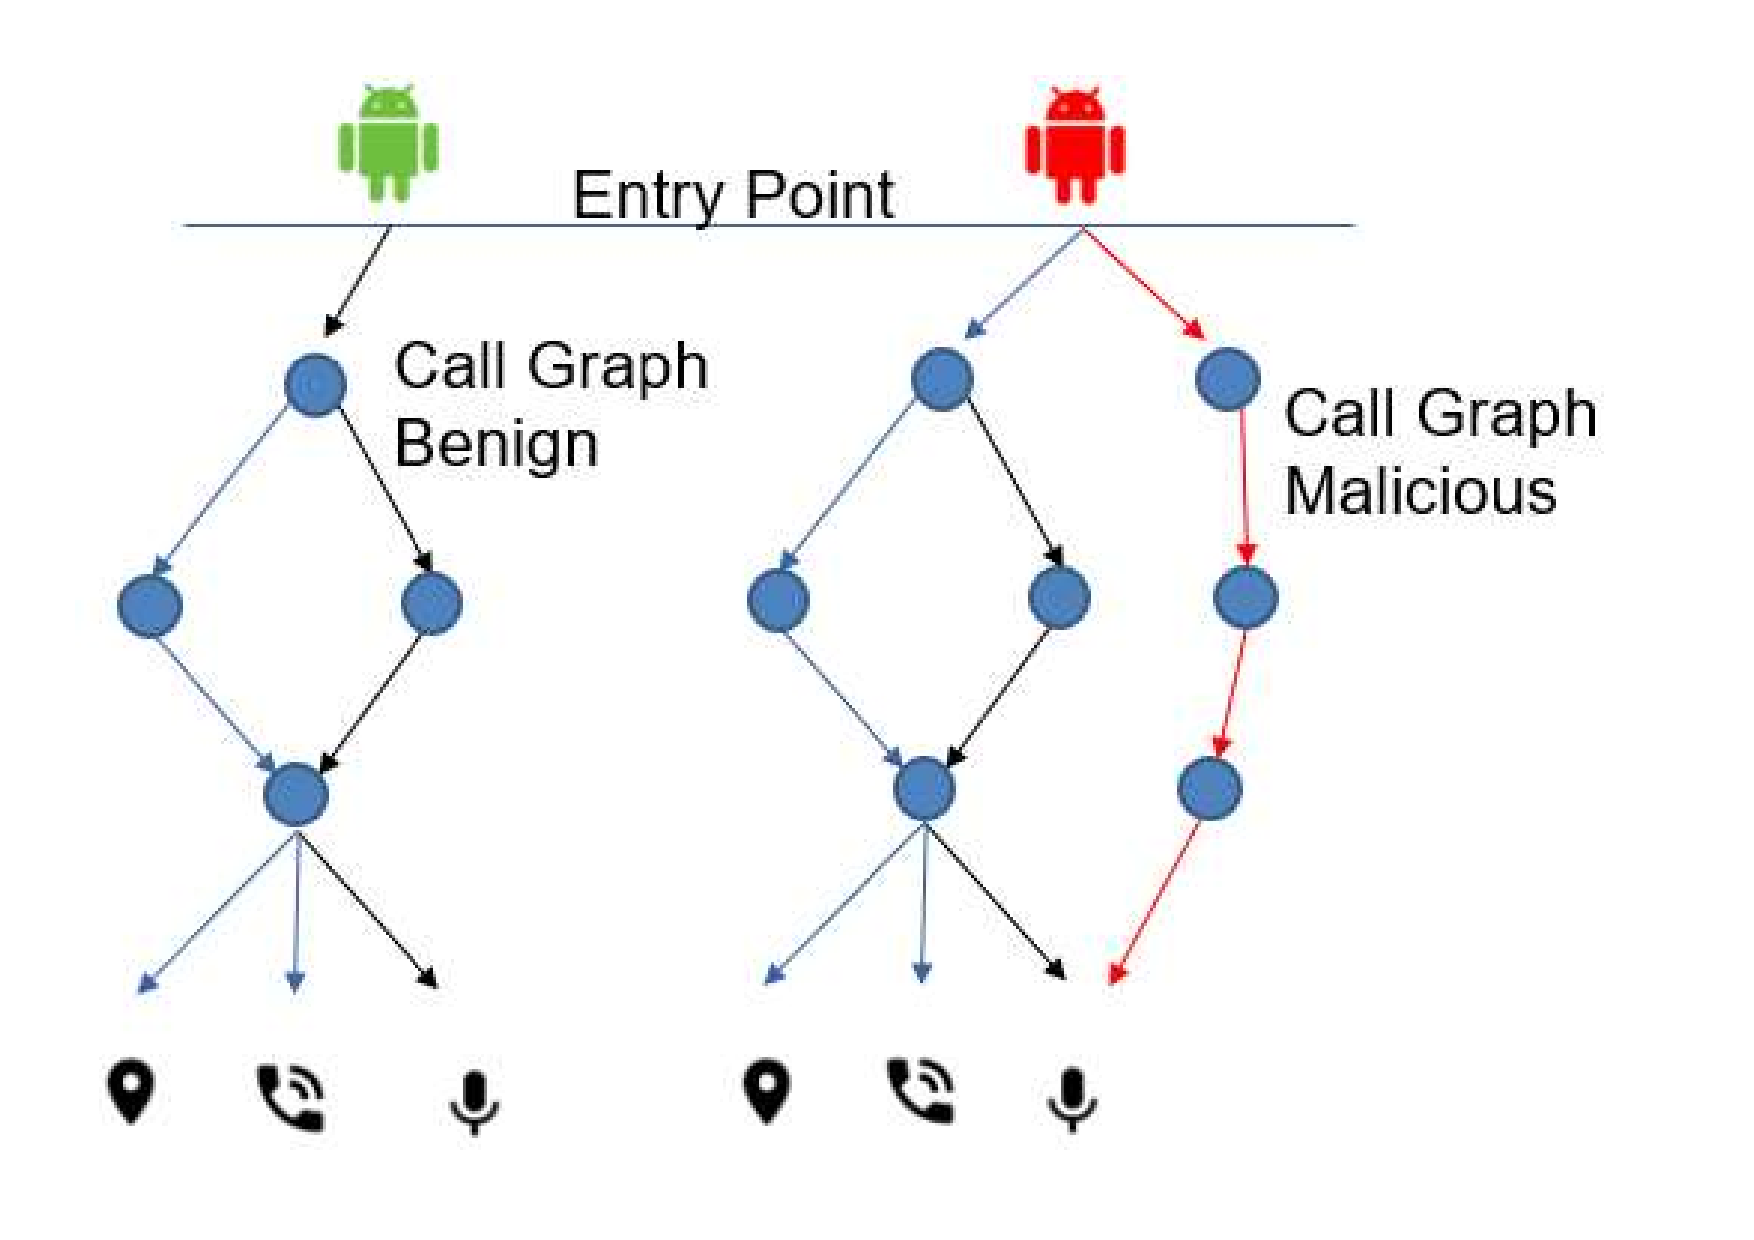
\includegraphics[scale=0.30]{images/maliciousCallGraph.pdf}
\caption{Illustrative example of the path analysis. In this case, both versions call the same set of sensitive APIs. Nonetheless,
the paths between the entry points and the calls to sensitive APIs diverge.}
 \label{fig:callGraph}
\end{figure}

\begin{figure}
\centering
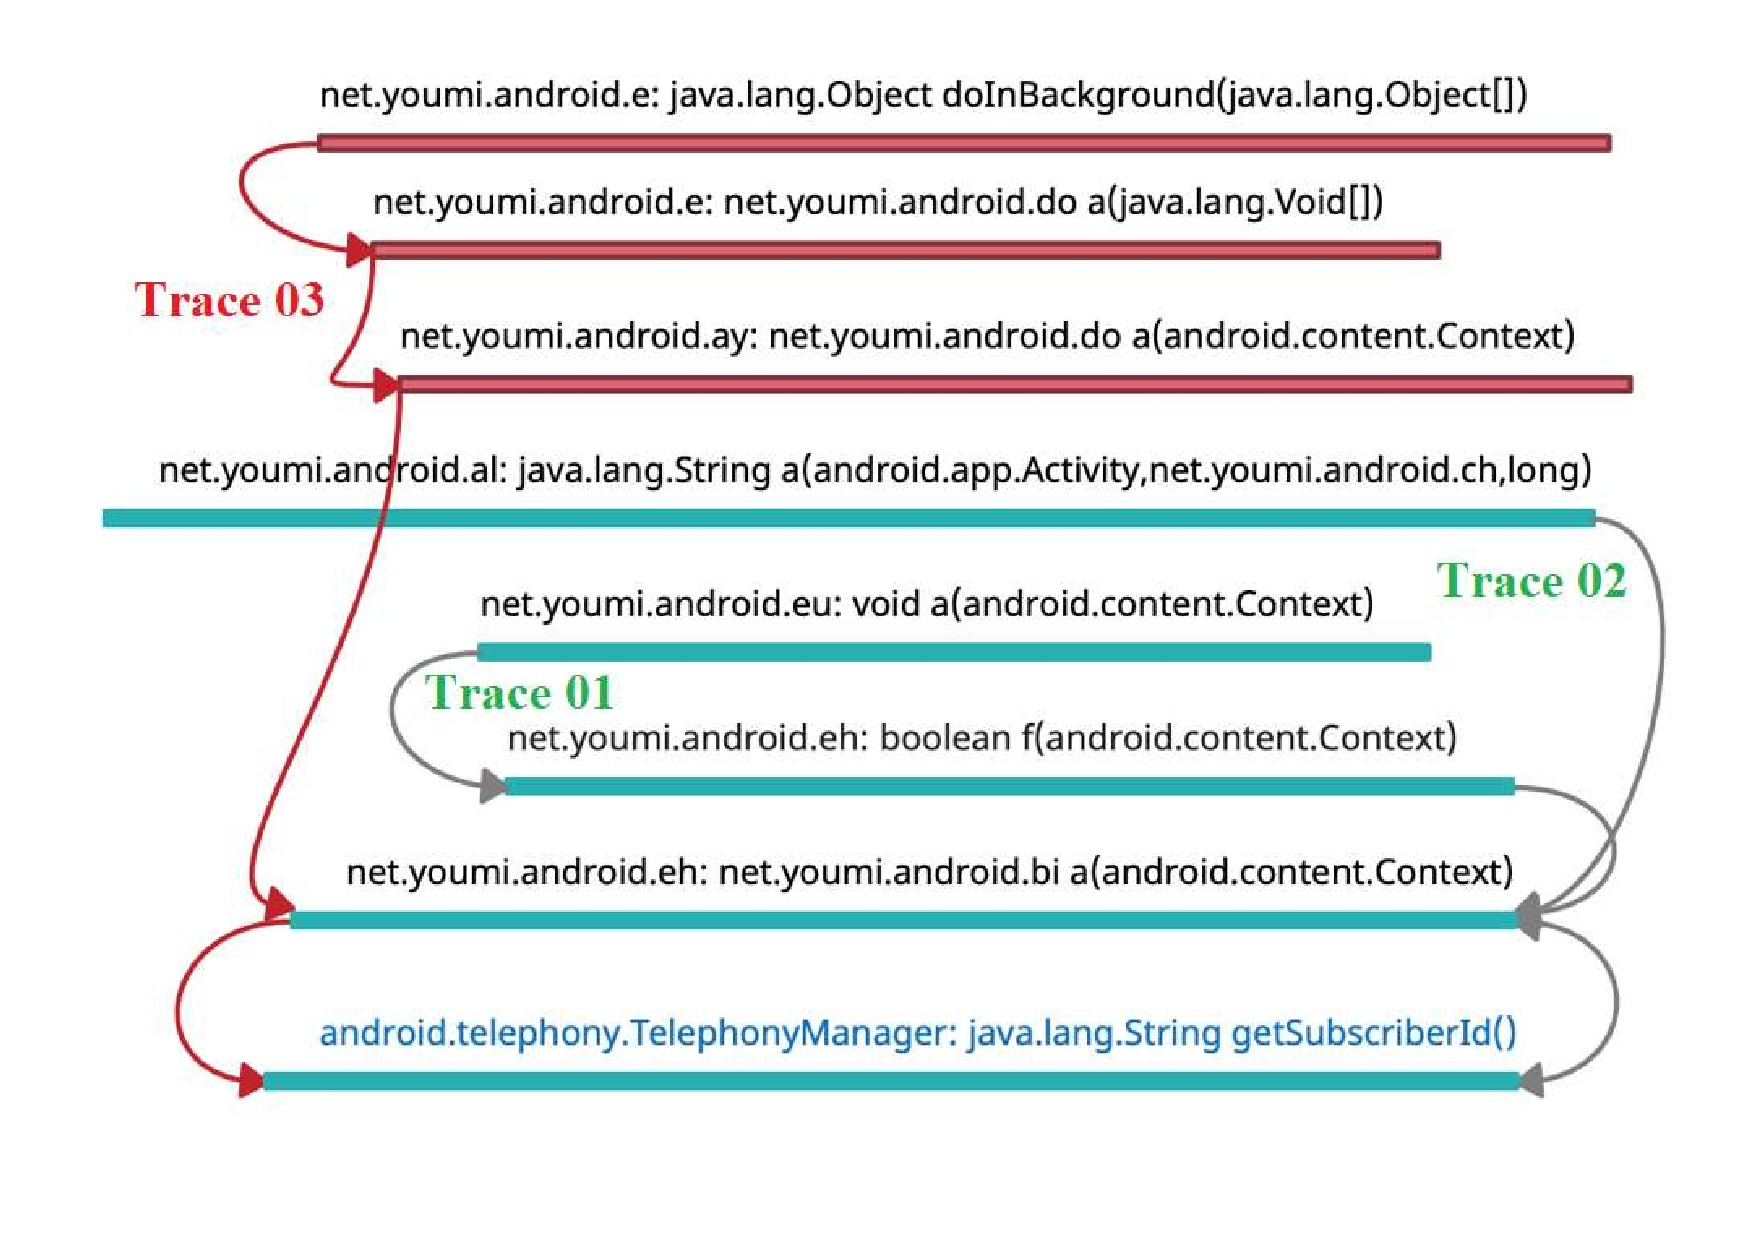
\includegraphics[scale=0.28]{images/maliciousTrace_example01.pdf}
\caption{Example of suspect path.}
 \label{fig:maliciousTrace}
\end{figure}

Recognizing that a malicious repackaged version of an app may exhibit the same set of calls
to sensitive APIs as the original, albeit with additional paths, we conducted an additional experiments
using all app pairs in our \cds. Our aim was to assess whether this path-based analysis extension could enhance
the accuracy of the \mas for malware classification. Our findings indicate that the inclusion of path analysis
leads to a modest reduction in false negatives, though, decreasing from 1,297 to 1,164.
However, this improvement comes at the expense of a slight increase in false positives, rising from 592 to 594
(as depicted in the first and third rows of Table~\ref{tab:accuracyParameter}).
In conclusion, the extension of path analysis enhances the overall accuracy ($F_1$) of the vanilla
\mas from 0.60 to 0.63.

\subsection{Parameter Analysis}

As described in~\cite{le2018towards}, malicious apps might require external data,
such as a remote server address to push advertisements, or sink sensitive information to another location,
different from the original version, using SMS messages (for instance). For this purpose, malicious apps
might change the actual parameter values used in calls to sensitive APIs, values that might differ from those
used in the original app. Thus, we hypothesize that differences on the parameter values (from both app versions), passed to the same calls to
sensitive APIS, might provide hints of suspiciously repackaged apps. Figure~\ref{fig:parameterDiff} presents a concrete example of
different parameter values used in the calls to the same sensitive method. This example comes from the \texttt{com.nla.downloader} app
(one of the apps in the \cds), and uses a \texttt{java.net.URL} object to remunerate a different publisher from the original app.
{\color{red}Although not expressly harmful, repackaged apps might use objects from this class to download and run external files
  from a network in the infected system~\cite{DBLP:journals/compsec/ObaidatSPP22}.} We executed our
experiment one more time, to estimate the impact of parameter analysis into the accuracy of the \mas for
malware detection. 
The parameter analysis reduces the number of false negatives from 1,297 (vanilla \mas) to 1,221, with the side effect of
increasing the number of false positives from 592 to 603 (see the first and second rows of Table~\ref{tab:accuracyParameter}).
In general, the accuracy ($F_1$) of the \mas using parameter analysis improves from 0.60 to 0.62 at \cds.

\begin{figure*}[t]
\centering
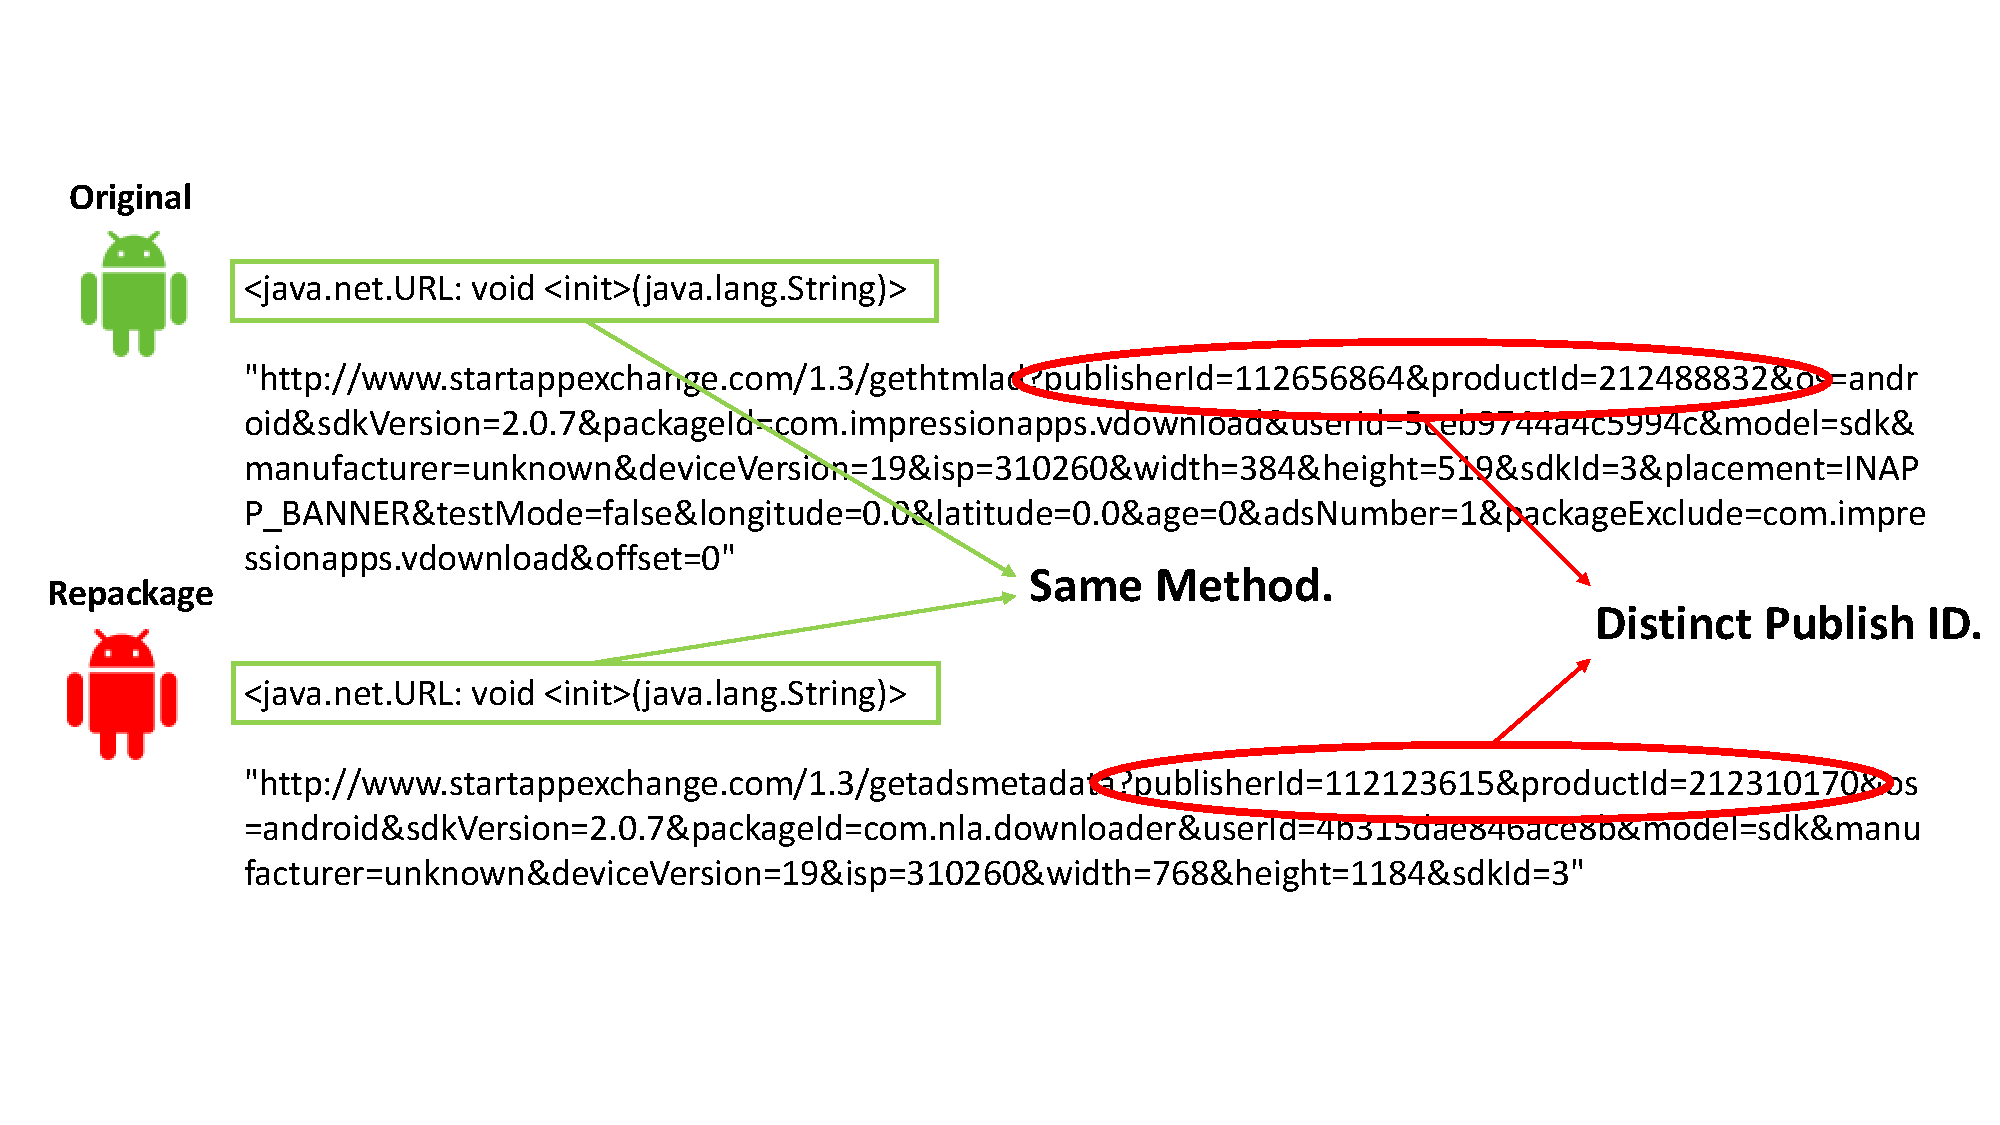
\includegraphics[scale=0.3]{images/parameterDiff.pdf}
\caption{Example of different parameter values used in the same method call.}
 \label{fig:parameterDiff}
\end{figure*}

\begin{table*}[ht]
  \caption{Accuracy of the \mas with aid of complementary techniques (3,211 app pairs).}
\centering{
  \begin{tabular}{lrrrrrr} \hline
    Dataset & TP   & FP  & FN  & Precision & Recall & $F_1$ \\ \hline
    
    %\mas + Traces  & \sds (102)   & 67   & 18  & 2   & 0.78      & 0.97   & 0.87  \\
    \cds \mas    & 1,422  & 592 & 1,297 & 0.70       & 0.52   & 0.60  \\
    \cds \mas + Trace     & 1,555  & 594 & 1,164 & 0.72       & 0.57   & 0.63  \\
    \cds \mas + Parameter     & 1,498  & 603 & 1,221 & 0.71       & 0.55   & 0.62  \\
    \cds \mas + Trace + Parameter     & 1,620  & 605 & 1,099 & 0.72       & 0.59   & 0.65  \\
    %\mas + Traces  & \cds (1203)   & 214  & 326 & 245 & 0.39      & 0.46   & 0.42  \\ 
    \hline
  \end{tabular}
  }
  \label{tab:accuracyParameter}
\end{table*}

\subsection{Combining The Path and Parameter-based extensions}

Finally, we investigate if we could benefit
from combining both extensions (path and parameter-based extensions).
The execution that combines both extensions correctly classifies 1,620 repackaged apps as malware (TP),
reducing the number of FN from 1,297 to 1,099. Nonetheless, this execution increases the number of FP from 592 to 605.
The combination of both techniques proves to be more effective than the vanilla \mas or when we use just one of the extensions.
In summary, the results of our last experiment reveal that the combination of both techniques presents an $F_1$ score of
0.65 (see Table 6).

\tb{5}{When combining both techniques, we reduces the number of false negatives (in comparison with the vanilla \mas), with the side effect of increasing the number of false positives. However, this configuration improves the
overall accuracy ($F_1$) of \mas at malware detection, from 0.60\% to 0.65\% at \cds.} 
